\section{Reconnaissance Platform}\label{sec:implementation_reconnaissance_platform}

Finally, to implement the reconnaissance platform, three main components are needed: video capture, video processing, and insights generation. The video capture component is responsible for capturing the video feed from the \gls{uav} camera. The video processing component is responsible for processing the video feed to extract relevant information. The insights generation component is responsible for generating insights from the processed video feed. Each different component is implemented separately and then integrated into the reconnaissance platform as a whole.

\subsection{Video Capture}\label{subsec:implementation_video_capture}

In order to capture the video from the Ricoh Theta X 360 Degree Camera \autocite{ricohimagingTHETARicoh}, the camera is connected to the NVIDIA Jetson Orin \autocite{nvidiaNVIDIAJetson} using a \gls{usb} C cable. The camera is configured to stream the video feed to the NVIDIA Jetson Orin using the Ricoh Theta X 360 Degree Camera API \autocite{ricoh360ReferenceRicoh}. In order to be able to capture the video feed from the camera, several libraries are used, such as OpenCV \autocite{githubGitHubOpencvopencv}, GSTThetaUVC \autocite{githubGitHubBuburidergstthetauvc}, LibUVC \autocite{githubGitHub6GIntegration3UC3Mlibuvcthetasample}, and V4L2 \autocite{githubGitHubUmlaeutev4l2loopback}. It is worth mentioning that the libraries used had to be modified to work with the Ricoh Theta X 360 Degree Camera, as it is not officially supported by the libraries. The video feed is captured in real-time and sent to the video processing component for further processing.

\todo{add some examples}

\subsection{Video Processing}\label{subsec:implementation_video_processing}

Once the video feed is captured by the Jetson Orin, it is further processed to extract relevant information. The video processing is done using deep learning algorithms to detect and track objects in the environment. The model used for the object detection and tracking is the YOLOv11 \autocite{ultralyticsYOLO11} as it is the defacto standard for object detection and tracking in real-time. It provides the best performance in terms of accuracy and speed, as well as being able to run on the Jetson Orin. The model used was the YOLOv11-medium with a pixel resolution of 640x640 px and an inference time of \SI{56}{\milli\second}. \todo{add script used to run everything}

\todo{add some examples}

\subsection{Insights Generation}\label{subsec:implementation_insights_generation}

Finally, all the detected and tracked objects are sent to the insights generation component to generate insights for the end-user. In order to process the detected and tracked objects, a web application was developed using the NextJS framework \autocite{nextjsNextjsVercel} for the backend, ReactJS \autocite{reactReact} for the frontend, Tailwind CSS \autocite{tailwindcssTailwindRapidly} for the styling, and Prisma \autocite{prismaPrismaSimplify} for the database hanldling. This web application is responsible for displaying the detected and tracked objects in real-time, as well as generating alerts and notifications in case of critical events or failures. The web application is also responsible for managing the different missions of the \glspl{uav} with the objectives and constraints defined by the end-user and also handling the user authentication and authorization.

The web application is divided into three main layers: the application layer, the presentation layer, and the data layer. The application layer is responsible for handling the business logic of the web application, such as the user authentication and authorization, the mission management, the rule management, the detection management, the alert management, and the notification management. The presentation layer is responsible for displaying the information to the end-user. The data layer is responsible for storing the information of the web application.

\subsubsection{Data Layer}\label{subsubsec:implementation_data_layer}
The data layers are divided into two main components: the object storage and the database. The object storage is used to store the video feed captured by the camera, as well as the detected and tracked objects. The object storage used was Amazon S3 \autocite{amazonCloudComputing}, as it provides a reliable and scalable storage solution for the web application.  For the database, a relational database was used to store the information of the web application. As Prisma \autocite{prismaPrismaSimplify} was used for the database handling, the database chosen can be any database supported by Prisma, such as PostgreSQL, MySQL, SQLite. This was chosen to provide flexibility and scalability to the system, as well as to be able to easily switch between databases if needed for different use cases such as testing, development, or production. The schema of the database can be seen in \cref{fig:database_schema}. The schema has six main tables, each one responsible for storing different information:

\begin{itemize}
  \item User: stores the information of the users of the system that can access the web application. It is used for user authentication and authorization purposes.

  \item Drone: stores the information of the drones that are connected to the system. It is used to manage the different drones and their missions. Each drone has a unique identifier, and a specific secret token to authenticate with the system and allow the drone to send the data to the system.

  \item Mission: stores the information of the missions of the drones. It is used to manage the different missions of the drones and group drones together for specific tasks. Each mission can be composed of one or more drones, and each drone can be part of one or more missions. Moreover, users are assigned to missions to have access to the data collected by the drones.

  \item Rule: stores the information of the rules of a specific mission to generate alerts and notifications. It is used to define the objectives and constraints of a mission, such as the specific objects to detect and track, the specific alerts to generate, and the specific notifications to send.

  \item Detection: stores the information of the detected objects in the environment by a drone for a specific mission. It is used to store the detected objects and their properties, such as the class, the confidence, the position, the size, and the orientation.

  \item Alert: stores the information of the alerts generated by the system for a specific mission created by a rule. It is used to store the alerts and their properties, such as the type, the severity, the message, the timestamp, and the status.
\end{itemize}

\begin{figure}
  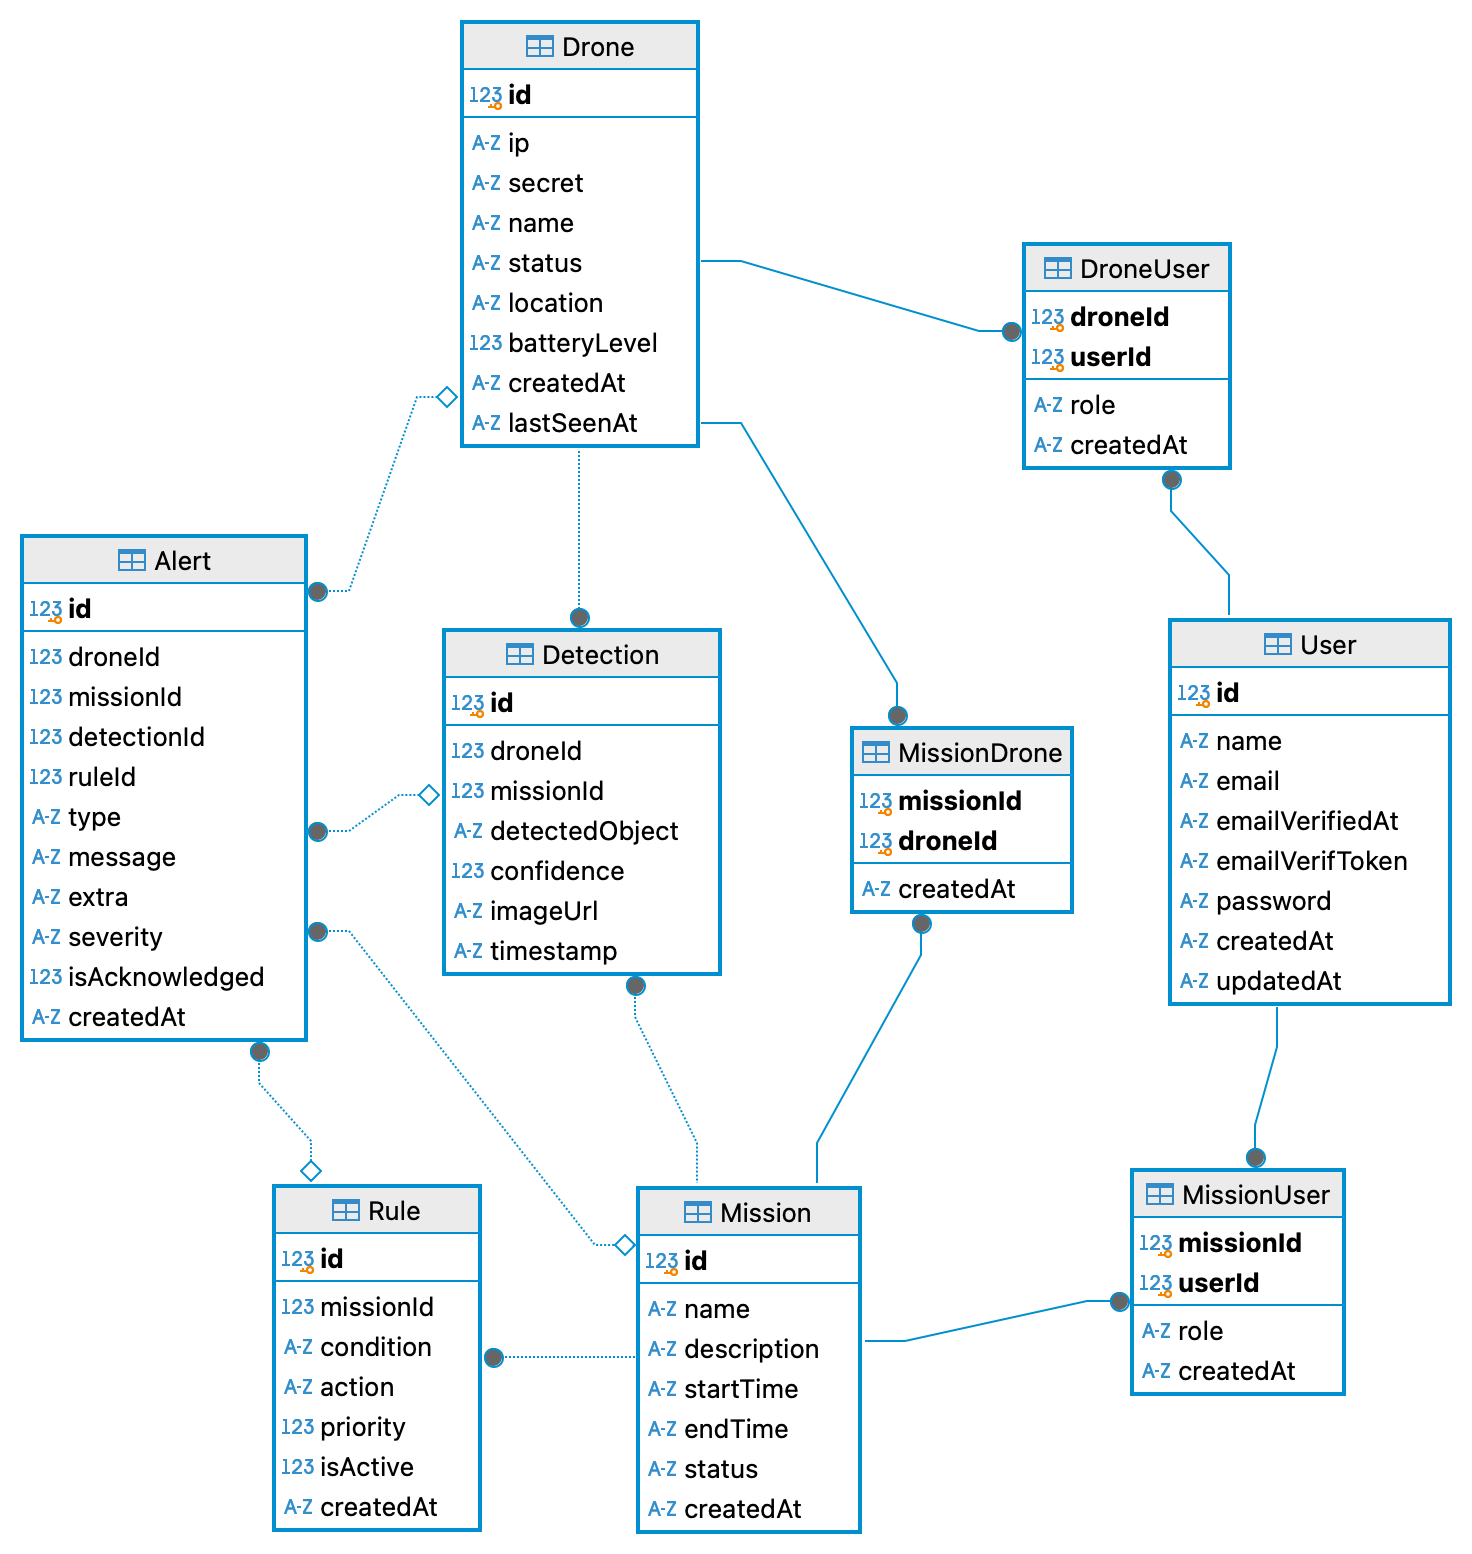
\includegraphics{reconnaissance_platform_database_schema.png}
  \caption{Database schema of the reconnaissance platform.}\label{fig:database_schema}
\end{figure}

\subsubsection{Presentation Layer}\label{subsubsec:implementation_presentation_layer}

The presentation layer is developed using the ReactJS framework \autocite{reactReact} for the frontend, Tailwind CSS \autocite{tailwindcssTailwindRapidly} for the styling, and Prisma \autocite{prismaPrismaSimplify} for the database handling. In order to provide a responsive and user-friendly interface, the web application is divided into different components, such as the login component, the dashboard component, the mission component, the drone component. Each component is responsible for displaying the information to the end-user and providing the necessary functionalities to interact with the system. The web application is designed to be easy to use and intuitive, as well as to provide real-time updates and notifications to the end-user. In \cref{fig:web_application}, a screenshot of the web application can be seen showcasing the dashboard component.

\todo{add screenshot of the web application}



\subsubsection{Application Layer}\label{subsubsec:implementation_application_layer}

% Local Variables:
% jinx-local-words: "defacto githubGitHubBuburidergstthetauvc githubGitHubOpencvopencv nvidiaNVIDIAJetson ricohimagingTHETARicoh uav"
% End:
